\chapter{Konstruktion}

Materialet der er valgt til konstruktionen er RK profil på grund af at de er lette at arbejde med og fordi de egner sig til formålet på grund af rillerne der er i profilerne. rillerne benyttes til bælterne som skal trække x og y akserne. 

Skitser til designet af den ydre og indre ramme blev udarbejdet. Vigtist for rammen var at standard vinflasken som er defineneret i bilag x kunne passe ind i den indre ramme.
Flaskens højde er ca 30 cm, og derfor var det nødvendigt at der fra åbningsmekanismens bund og til flaskehalsens top minimum skal være 30 cm. Derfor er det valgt at den ydre rammes mål skal være minimum 50 cm.

Den ydre ramme ses illustreret på figur \ref{CT_CD}.

\begin{figure}[H]
	\centerline{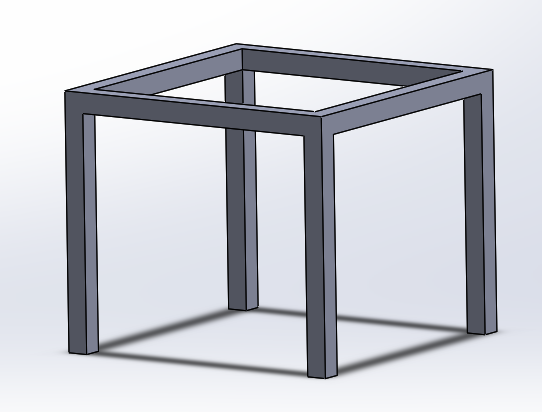
\includegraphics[scale=1]{Konstruktion/Billeder/ydre_ramme}}
	\caption{Ydre ramme}
	\label{CT_CD}
\end{figure}

\noindent
Den ydre ramme består af 8 500 mm rk profiler. Profilerne har en dimmension på 40x40 mm.\\

Den indre ramme består af 4x400 mm lange RK profiler. De er sat sammen med trekantede beslag. I 2 af beslagene er der borret 8 mm gevind huller, mens de 2 andre blot er 8 mm huller. De to gevindhuller er lavet således at bevægelsen på z-aksen kan ske ved at 2 motorer skruer 2 gevindstænger ind og ud af de 2 gevindhuller.

En illustration af den indre ramme kan ses på figur \ref{IR}.

\begin{figure}[H]
	\centerline{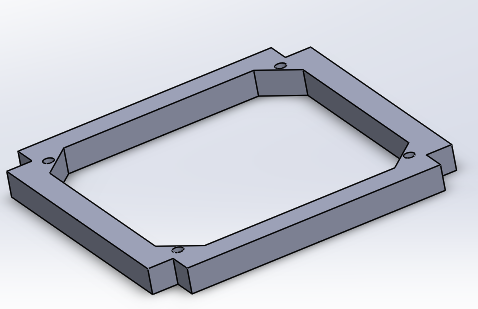
\includegraphics[scale=1]{Konstruktion/Billeder/indre_ramme}}
	\caption{Indre ramme}
	\label{IR}
\end{figure}

\noindent
X-aksen består af en 480 mm lang RK profil som lægges vandret over den indre ramme. Denne bliver trukket ved hjælp af bælter som er monteret på profilen. På denne profil er en sensor og en refleks montoret således det er muligt at detekter når vinen er indsat i WinPrep. Sensorens placering er markeret med blå mens refleksens placering er markeret med rød på figur \ref{XA}.

\begin{figure}[H]
	\centerline{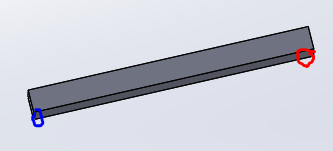
\includegraphics[scale=1]{Konstruktion/Billeder/x_akse}}
	\caption{X-akse}
	\label{XA}
\end{figure}
	
\noindent
For at y-aksen ikke rammer ind i x-aksen er den løftet 10 cm over. Detter er gjort med 10 cm lange RK profiler. 
På figur \ref(YA) ses y-aksen.

\begin{figure}[H]
	\centerline{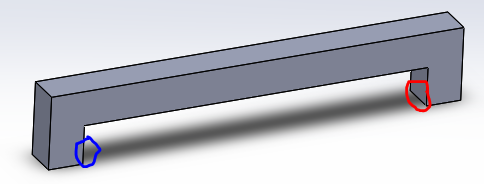
\includegraphics[scale=1]{Konstruktion/Billeder/y_akse}}
	\caption{Y-akse}
	\label{XA}
\end{figure}

\noindent
For at åbningsmekanismen kan bevæge sig rigtigt i forhold til akserne er der lavet et beslag som er sat til begge akse. Dette beslag trækker x-aksen med sig når y-aksen bevæger sig og omvendt. på nuværrende tidspunkt er der ikke implementeret en åbningsmekanisme, og derfor er den blot lavet som en cylinder.

Beslaget med åbningsmekanismen ses på figer \ref{BS}.

\begin{figure}[H]
	\centerline{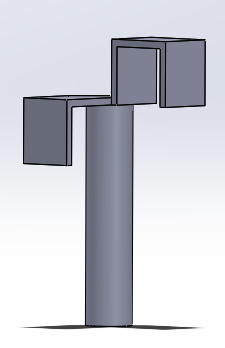
\includegraphics[scale=1]{Konstruktion/Billeder/bs}}
	\caption{Beslag med åbningsmekanisme}
	\label{XA}
\end{figure}

\noindent
Samlet skal den indre ramme løftes af 2 gevindstænger og to glatte stænger som er sat fast i den ydre ramme.

Den indre ramme med gevind og glattestænger ser ud som på figur \ref{IR_F}.

\begin{figure}[H]
	\centerline{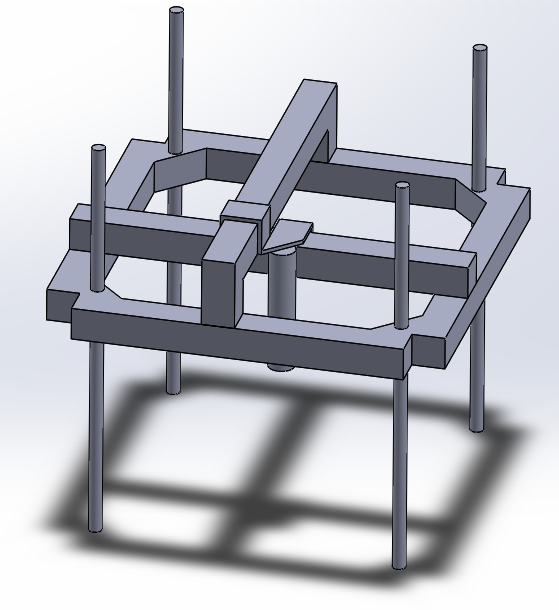
\includegraphics[scale=1]{Konstruktion/Billeder/IR_F}}
	\caption{Den samlede indre ramme.}
	\label{IR_F}
\end{figure}

\noindent
Når det hele sættes sammen ser det ud som på figur \ref{FR}.

\begin{figure}[H]
	\centerline{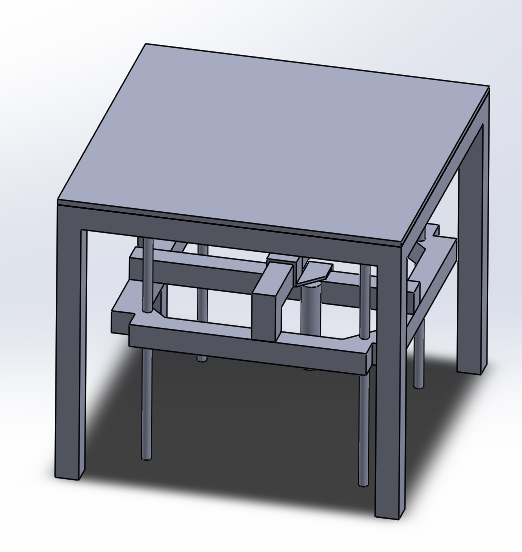
\includegraphics[scale=1]{Konstruktion/Billeder/fr}}
	\caption{Den samlede indre ramme.}
	\label{FR}
\end{figure}